%!TEX root = ../main.tex
\documentclass[../main]{subfiles}

\begin{document}

% \footnotesize
% \begin{longtable}[H]{|c|c|c|c|c|c|}
%     \caption{Групповая матрица попарных сравнений <<Стоимость про\-из\-вод\-ства>>\label{tab:gmanufacture_cost}}\\\hline
%     \multicolumn{1}{|c|}{\makebox[1.5cm]{$E   $}} &
%     \multicolumn{1}{c|} {\makebox[1.5cm]{$S_{5}  $}} &
%     \multicolumn{1}{c|} {\makebox[1.5cm]{$S_{8}  $}} &
%     \multicolumn{1}{c|} {\makebox[1.5cm]{$S_{18} $}} &
%     \multicolumn{1}{c|} {\makebox[1.5cm]{$S_{19} $}} &
%     \multicolumn{1}{c|} {\makebox[1.5cm]{$S_{20} $}} \\\hline
%     \endfirsthead
%     \caption*{Продолжение таблицы \ref{tab:gmanufacture_cost}}\\\hline
%     \multicolumn{1}{|c|}{\makebox[1.5cm]{$E   $}} &
%     \multicolumn{1}{c|} {\makebox[1.5cm]{$S_{5}  $}} &
%     \multicolumn{1}{c|} {\makebox[1.5cm]{$S_{8}  $}} &
%     \multicolumn{1}{c|} {\makebox[1.5cm]{$S_{18} $}} &
%     \multicolumn{1}{c|} {\makebox[1.5cm]{$S_{19} $}} &
%     \multicolumn{1}{c|} {\makebox[1.5cm]{$S_{20} $}} \\\hline
%     \endhead
%     \endfoot
%     \endlastfoot
%     $S_{5}  $ & $1.00$ & $6.70$ & $8.49$ & $0.21$ & $2.45$ \\\hline
%     $S_{8}  $ & $0.15$ & $1.00$ & $0.35$ & $0.15$ & $0.31$ \\\hline
%     $S_{18} $ & $0.12$ & $2.83$ & $1.00$ & $0.12$ & $1.00$ \\\hline
%     $S_{19} $ & $4.73$ & $6.74$ & $8.21$ & $1.00$ & $6.96$ \\\hline
%     $S_{20} $ & $0.41$ & $3.22$ & $1.00$ & $0.14$ & $1.00$ \\\hline
% \end{longtable}
% \normalsize

% \begin{landscape}
%     \begin{figure}[H]
%         \centering
%         \ffigbox[\FBwidth]
%         {\caption{Иерархия критериев\label{fig:hierarchy}}}
%         {\includegraphics[width=\textwidth]{pic.pdf}}
%         \vspace{-14pt}
%     \end{figure}
% \end{landscape}


\newpage
\section{Анализ предметной области}

\subsection{Статистические модели текстовых документов}

Были протестированы две модели векторизованного представления текста -- <<мешок слов>> и модель TF-IDF. Модель <<мешок слов>> представляет документ в виде матрицы, представленной на рисунке \ref{fig:bow}. Здесь слова каждого абзаца подсчитываются и сопоставляются с абзацами, в которых они встретились.

\begin{figure}[H]
    \centering
    \ffigbox[\FBwidth]
    {\caption{Bag-of-Words матрица\label{fig:bow}}}
    {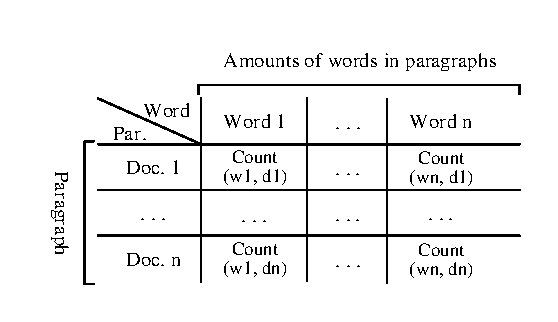
\includegraphics[width=.7\textwidth]{1.pdf}}
    \vspace{-\baselineskip}
\end{figure}


Модель TF-IDF представляет документ в виде матрицы, представленной на рисунке \ref{fig:tfidf}. Формула (\ref{eq:tfidf}) показывает, как можно получить метрику TF-IDF.
\begin{equation}
    \label{eq:tfidf}
    tfidf(t, d, D) = \frac{n_t}{\displaystyle\sum_k n_k} \times 
    log \frac{ \big|{D}\big| }
    { \big|\left\{ d_i \in D : t \in d_i \right\}\big| }\ ,
\end{equation}
\makebox[12.5mm]{где\hfill}$t$ -- термин или слово;\\
\makebox[12.5mm]{}$d$ -- конкретный абзац;\\
\makebox[12.5mm]{}$D$ -- набор абзацев. 

Итак, модель TF-IDF придает больший вес словам которые использованы меньше раз. Это может быть полезно, когда тексты схожи с точки зрения используемых слов, как в нашем случае, для политик безопасности.

\begin{figure}[H]
    \centering
    \ffigbox[\FBwidth]
    {\caption{Матрица TF-IDF\label{fig:tfidf}}}
    {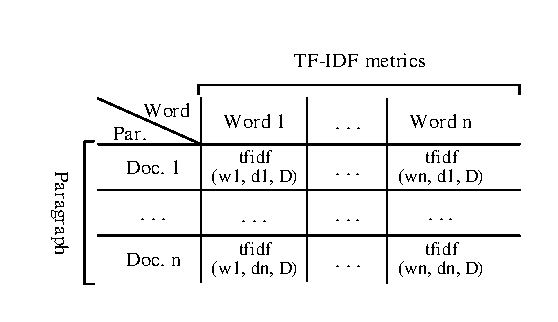
\includegraphics[width=.7\textwidth]{2.pdf}}
    \vspace{-\baselineskip}
\end{figure}

\subsection{Подход основанный на латентно-семантическом анализе текста}

Современные методы кластеризации текстов позволяют определять тематику текстов с высокой точностью. Однако большинство из этих методов принимают тексты с самыми разными темами как вход для алгоритмов. Но тексты со схожими тематиками можно проанализировать с помощью ла\-тен\-тно-семантического анализа дважды: группировать тексты по темам один раз, и предоставить еще более детальное разделение их по подтемам во второй раз. Такой подход можно использовать для более точной классификации абзацев с точки зрения их характеристик и аспектов использования персональных данных. Следует отметить, что латентно-семантический поиск сильно зависит от глобального текстового контекста с потерями информации о локальных контекстных отношениях между словами. Были выделены девять тем конфиденциальности, которые следует сопоставить с абзацами согласия пользователя сайта -- <<сбор личных данных>>, <<сбор данных третьими лицами>>, <<управление личными данными>>, <<механизмы защиты персональных данных>> и др. Очевидно, что аспекты обращения с данными состоят из нескольких слов, и в некоторых случаях перекрываются. На основании этих фактов была выдвинута гипотеза о том, что латентно-семантический поиск способен обнаружить даже незначительную разницу в тексте абзацев при пропуске частых слов. Перед применением латентно-семантического анализа требуется предварительная обработка входных данных. Обычно эта процедура включает очистку данных, удаление гиперссылок, пунктуации и т. д. Также текст политик конфиденциальности был разбит на набор абзацев. Каждый абзац был преобразован в массив слов, которые он содержит. Следующим шагом было удаление наиболее частых, но не столь значимых слов, так называемых стоп-слов. Также была применена операция стемминга, чтобы рассматривать только основную часть всех слов полученных от единого корня.

Пусть A -- это матрица абзацев и слов, тогда используя формулу (\ref{eq:lsa})
\begin{equation}
    \label{eq:lsa}
    A = U \times S \times V^T
\end{equation}
\makebox[12.5mm]{где\hfill}$A$ -- матрица слов и параграфов;\\
\makebox[12.5mm]{\hfill}$U$ -- ортонормированная матрица $U$;\\
\makebox[12.5mm]{\hfill}$V$ -- ортонормированная матрица $V$;\\
\makebox[12.5mm]{\hfill}$S$ -- диагональная матрица $S$, значения которой сингулярны для $A$.

После того, как матрица была разделена на три компонента, матрица $U$ содержит $n$-мерные векторы, которые можно интерпретировать как координаты в $n$-мерном пространстве \cite{LSA}. Документы могут быть распределены по кластерам по значениям этих координат. Проведенные эксперименты с латентно-семантическим анализом выполнялись с использованием набора данных с открытым исходным кодом, который включает 115 политик безопасности, которые были размечены вручную, и все абзацы присвоены одному или нескольким сценариям использования персональных данных \cite{OPP}. Результаты экспериментов для модели <<мешок слов>> представлены в таблице \ref{tab:clusters1}, в ней показаны полученные кластеры и соответствующие значения координат.

\begin{longtable}[H]{|l|l|l|l|l|}
    \caption{Кластеры политик безопасности для модели Bag-of-Words\label{tab:clusters1}}\\\hline
    \multicolumn{1}{|c|}{№} & 
    \multicolumn{1}{c|}{Coordinate 1} & 
    \multicolumn{1}{c|}{Coordinate 2} & 
    \multicolumn{1}{c|}{Coordinate 3} & 
    \multicolumn{1}{c|}{Coordinate 4} \\
    \hline
    \endfirsthead
    \caption*{Продолжение таблицы \ref{tab:clusters1}}\\\hline
    \multicolumn{1}{|c|}{№} & 
    \multicolumn{1}{c|}{Coordinate 1} & 
    \multicolumn{1}{c|}{Coordinate 2} & 
    \multicolumn{1}{c|}{Coordinate 3} & 
    \multicolumn{1}{c|}{Coordinate 4} \\
    \endhead
    \endfoot
    \endlastfoot
    0 & 0.634”inform”  & 0.28”may”        & 0.276”use”     & 0.232”servic”   \\\hline
    1 & 0.202“cooki”   & 0.466“inform”    & 0.336“site”    & 0.257“use”      \\\hline
    2 & 0.524“privaci” & 0.433“polici”    & 0.388“cooki”   & 0.219“site”     \\\hline
    3 & -0.589“servic” & 0.344“site”      & 0.244“parti”   & -0.240“third”   \\\hline
    4 & -0.504“parti”  & 0.486 “third”    & -0.449“servic” & 0.235“advertis” \\\hline
    5 & -0.594“site”   & 0.278“cooki”     & 0.272“websit”  & 0.264“privaci”  \\\hline
    6 & -0.326“may”    & 0.311“site”      & 0.307“servic”  & -0.293”email”   \\\hline
    7 & -0.437”may”    & -0.369”advertis” & 0.345”person”  & 0.319”cooki”    \\\hline
    8 & 0.501”may”     & -0.315”email”    & -0.281”use”    & -0.264”address” \\\hline
    9 & -0.488”user”   & -0.384”use”      & 0.310”provid”  & -0.301”websit”  \\\hline
\end{longtable}

Как видно, результаты противоречивы, поэтому трудно понять, какая из тем каким смыслом обладает. Затем рассчитывалась метрика принадлежности к теме с помощью библиотеки Gensim \cite{Gensim} и результаты снова не были обнадеживающими. Результаты расчета метрики принадлежности кластеру представлены в таблице \ref{tab:affiliation_bow1}.

\begin{longtable}[H]{|c|c|c|c|c|c|}
    \caption{Принадлежность кластерам\label{tab:affiliation_bow1}}\\\hline
    \endfirsthead
    \endhead
    \endfoot
    \endlastfoot
    Topic       & 0     & 1     & 2    & 3     & 4     \\\hline
    Affiliation & 2.27  & -0.8  & 0.15 & -0.22 & -1.2  \\\hline
    Topic       & 5     & 6     & 7    & 8     & 9     \\\hline
    Affiliation & -0.17 & -0.15 & -0.2 & 0.22  & -0.07 \\\hline
\end{longtable}

Другие результаты с параграфами, относящимися к другому аспекту обращения с данными, были почти такими же. Результаты
представлены в таблице \ref{tab:affiliation_bow2}.

\begin{longtable}[H]{|c|c|c|c|c|c|}
    \caption{Принадлежность кластерам\label{tab:affiliation_bow2}}\\\hline
    \endfirsthead
    \endhead
    \endfoot
    \endlastfoot
    Topic       & 0    & 1     & 2    & 3    & 4    \\\hline
    Affiliation & 2.59 & -0.76 & 0.64 & 0.74 & 0.13 \\\hline
    Topic       & 5    & 6     & 7    & 8    & 9    \\\hline
    Affiliation & 0.14 & -0.12 & 0.23 & 0.12 & 0.41 \\\hline
\end{longtable}

Все протестированные абзацы были сопоставлены с кластером 0, что не может быть верным так как абзацы относились к заведомо разным аспектам обращения с персональными данными. 

Результаты экспериментов для модели TF-IDF представлены далее, в таблице \ref{tab:clusters2}. Также показывались десять кластеров и значения атрибутов. И, как в первом случае с <<мешком слов>>, по значениям координат невозможно судить о теме кластера.

\begin{longtable}[H]{|l|l|l|l|l|}
    \caption{Кластеры политик безопасности для модели Bag-of-Words\label{tab:clusters2}}\\\hline
    \multicolumn{1}{|c|}{№} & 
    \multicolumn{1}{c|}{Coordinate 1} & 
    \multicolumn{1}{c|}{Coordinate 2} & 
    \multicolumn{1}{c|}{Coordinate 3} & 
    \multicolumn{1}{c|}{Coordinate 4} \\
    \hline
    \endfirsthead
    \caption*{Продолжение таблицы \ref{tab:clusters2}}\\\hline
    \multicolumn{1}{|c|}{№} & 
    \multicolumn{1}{c|}{Coordinate 1} & 
    \multicolumn{1}{c|}{Coordinate 2} & 
    \multicolumn{1}{c|}{Coordinate 3} & 
    \multicolumn{1}{c|}{Coordinate 4} \\
    \endhead
    \endfoot
    \endlastfoot
    0 & 0.202“cooki”     & 0.2“may”        & 0.198“inform”   & 0.198“site”     \\\hline
    1 & 0.573“cooki”     & 0.262“browser”  & 0.195“advertis” & 0.182“web”      \\\hline
    2 & -0.406“media”    & 0.291“cooki”    & 0.282“health”   & 0.279“advertis” \\\hline
    3 & -0.453“health”   & 0.258“email”    & -0.204“kaleida” & 0.191“address”  \\\hline
    4 & 0.423“health”    & 0.215“media”    & 0.205“kaleida”  & -0.199“secur”   \\\hline
    5 & -0.299“advertis” & 0.262“health”   & -0.252“media”   & -0.213“privaci” \\\hline
    6 & -0.325“media”    & 0.263“polici”   & 0.249“privaci”  & 0.197”chang”    \\\hline
    7 & 0.280”cooki”     & -0.216”device”  & -0.183”health”  & -0.166”social”  \\\hline
    8 & -0.223”advertis” & -0.206”teenag”  & -0.206”inelig”  & 0.176”child”    \\\hline
    9 & -0.263” child”   & -0.26”wireless” & 0.245”message”  & 0.239”parent”   \\\hline
\end{longtable}

Результаты кластеризации снова противоречивы, поэтому трудно сказать, какая конкретная тема описывает какой аспект политики конфиденциальности. В разных темах встречаются одни и те же слова с изменение веса. Для аспектов политики конфиденциальности, которые мы искали нет тем, которые могли бы их точно описать, поскольку многие из них могут. Затем с помощью библиотеки Gensim был рассчитан показатель принадлежности к теме, и результаты снова не были обнадеживающими. Результаты расчета аффилированности по абзацу одной из политик конфиденциальности представленные в таблице \ref{tab:affiliation_tfidf1}.

\begin{longtable}[H]{|c|c|c|c|c|c|}
    \caption{Принадлежность кластерам\label{tab:affiliation_tfidf1}}\\\hline
    \endfirsthead
    \caption*{Продолжение таблицы\ref{tab:affiliation_tfidf1}}\\\hline
    \endhead
    \endfoot
    \endlastfoot
    Topic       & 0    & 1     & 2     & 3     & 4     \\\hline
    Affiliation & 2.18 & -0.97 & -0.69 & -0.27 & 0.65  \\\hline
    Topic       & 5    & 6     & 7     & 8     & 9     \\\hline
    Affiliation & 0.98 & -1.17 & 0.8   & 0.27  & 0.01  \\\hline
\end{longtable}

Результат для другого абзаца, относящегося к другой политике конфиденциальности, был почти такой же. Результаты представлены в таблице \ref{tab:affiliation_tfidf2}.

\begin{longtable}[H]{|c|c|c|c|c|c|}
    \caption{Принадлежность кластерам\label{tab:affiliation_tfidf2}}\\\hline
    \endfirsthead
    \caption*{Продолжение таблицы \ref{tab:affiliation_tfidf2}}\\\hline
    \endhead
    \endfoot
    \endlastfoot
    Topic       & 0    & 1    & 2     & 3     & 4     \\\hline
    Affiliation & 1.82 & 0.25 & 0.49  & 0.29  & -0.04 \\\hline
    Topic       & 5    & 6    & 7     & 8     & 9     \\\hline
    Affiliation & 0.74 & 0.52 & -0.04 & -0.58 & -1.33 \\\hline
\end{longtable}

Как можно заметить, результаты для модели TF-IDF аналогичны результатам модели <<мешка слов>>, за исключением нескольких незначительных изменений. Все абзацы снова были сопоставлены с кластером 0, что неверно, потому что они на самом деле описывают разные сценарии использования персональных данных. Эти эксперименты позволили сделать вывод, что использование латентно-семантического анализа не дает ценной информации о содержании онлайн-согласия пользователя. Проблема может быть связана с тем, что сценарии использования персональных данных очень похожи между собой, и для того, чтобы различать разные сценарии необходимо учитывать локальный контекст.

В результате апробации алгоритма латентно-семантического анализа было выяснено что для кластеризации экстремально схожих между собой текстов он  подходит не лучшим образом. В связи с этими обстоятельствами было решено обратить внимание на несколько иной подход анализа текста, основанный на контекстно-свободных грамматиках, тегировании по частям речи и синонимическом поиске.

\subsection{Подход основанный на латентном размещении Дирихле}

\subsection{Подход основанный на применении контекстно-свободных грамматик и синонимическом поиске}

Другой предложенный подход -- подход, основанный на анализе с помощью контекстно-свободных грамматик и синонимического поиска. Синонимический поиск в данном случае -- это подмена ключевых слов и их синонимов метками, например <<\_\_FP\_A\_\_>> означает, что это слово и его синонимы считаются акторами первой стороны. Этот метод можно применить ко многим другим словам. Например, сообщения электронной почты, аватары, местоположение также могут быть объектами и синонимами абстрактной метки <<\_\_CN\_\_>>, которая означает существительное сбора или объект сбора. Так все ключевые слова могут быть преобразованы в их смыслы в контексте предметной области. Маркировка выполняется легко, все слова совпадающие с пулами заменяются метками этих пулов.

Предварительная обработка данных в данном случае состоит из токенизации и лемматизации для более гибкой замены слов на метки их пулов.

При анализе пользовательского согласия сайта недостаточно найти ключевые слова, относящиеся к разным типам персональных данных, например цель и правовую основу распознать гораздо сложнее. Следующий шаг - установить слова отношения в предложениях, чтобы можно было определенно сказать, что ярлыки пулы синонимов связаны друг с другом и формируют логическая цепочку. Один из возможных способов определения отношений слов в тексте на естественном языке -- это синтаксический анализ предложения, основанный на частеречной разметке \cite{POS}. Имея размеченное по частям речи предложение, парсер грамматики NLTK \cite{NLTK} строит деревья предложений по правилам грамматики. Одно из таких деревьев в обозначениях NLTK можно увидеть на рисунке \ref{fig:nltk_tree} \cite{NLTK}, где <<S>> -- основа предложения, <<NP>> -- именная фраза, <<VP>> -- глагольная фраза, <<Adj>> -- прилагательное, <<НОМ>> -- именное словосочетание, <<ПП>> -- предлог фраза, <<Det>> -- артикль, <<V>> -- глагол, <<N>> -- существительное, <<P>> -- предлог.

\begin{figure}[H]
    \centering
    \ffigbox[\FBwidth]
    {\caption{Матрица TF-IDF\label{fig:nltk_tree}}}
    {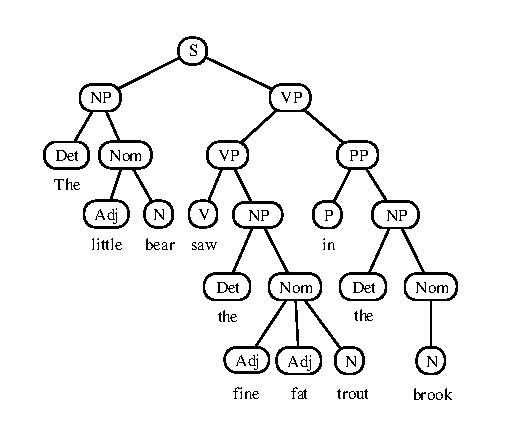
\includegraphics[width=.7\textwidth]{3.pdf}}
    \vspace{-\baselineskip}
\end{figure}

В предлагаемом подходе немного другая грамматическая запись. Созданная грамматика представлена в (\ref{eq:grammar1}).
\begin{equation}
    \label{eq:grammar1}
    \left\{ 
        \begin{array}{l}
            D \rightarrow S\ |\ S\ D\ |\ S\ \ U\ D\ \\
            S \rightarrow NPG\ \ \ VBG \\
            VPG \rightarrow VP\ |\ VP\ \ VPG\ |\ VP\ \ U\ \ VPG \\
            NPG \rightarrow NP\ |\ NP\ \ NPG\ |\ NP\ \ U\ \ NPG \\
            AJPG \rightarrow AJ\ |\ AJ\ \ APG\ |\ AJ\ \ U\ \ APG \\
            AVPG \rightarrow AV\ |\ AV\ \ APG\ |\ AV\ \ U\ \ APG \\
            VP \rightarrow V APG\ |\ V\ \ PPG\ |\ V\ \ PP\ \ APG \\
            NP \rightarrow NOM\ |\ DET\ \ NOM \\
            NOM \rightarrow N\ |\ AJPG\ \ N \\
            PP \rightarrow NPG\ |\ P\ \ NPG
        \end{array}
    \right.\ ,
\end{equation}
где <<D>> -- документ, <<S>> -- предложение, <<NPG>> -- группа именных фраз, <<VPG>> -- группа глагольных фраз, <<AJPG>> --  группа прилагательных, <<AVPG>> -- группа наречий, <<VP>> -- глагольная фраза, <<NP>> -- именная фраза, <<NOM>> -- именная фраза, <<PP>> -- предлог, <<DET>> -- артикль. Грамматика из формулы (\ref{eq:grammar1}) позволяет рекурсивно выделять основу предложения и последовательности глагола, существительного, прилагательного, наречия и т.д. Это все еще не идеальное решение, но попытка найти более сложные предложения в политиках безопасности. Этот подход требует использования пулов синонимов, которые соответствуют различным ключевым словам. Поэтому в грамматику включены метки пулов синонимов, привязанных к части речи. Метки пулов вручную назначены частям речи для преобразования привязок частей речи NLTK, это показано в формуле (\ref{eq:grammar2}).
\begin{equation}
    \label{eq:grammar2}
    \left\{ 
        \begin{array}{l}
            U \rightarrow NLTK\_CC \\
            DET \rightarrow NLTK\_DT \\
            AJ \rightarrow NLTK\_JJ \\
            AV \rightarrow NLTK\_RB \\
            N \rightarrow \_\_CN\_\_\ |\ \_\_FP\_A\_\_\ |\ \_\_TP\_A\_\_\ |\ NLTK\_N \\
            V \rightarrow \_\_CV\_\_\ |\ NLTK\_V
        \end{array}
    \right. 
\end{equation}
Здесь в формуле (4) <<NLTK\_CC>> -- соединение NLTK, <<NLTK\_N>> -- все формы существительных NLTK, <<NLTK\_В>> -- все формы глаголов NLTK, <<NLTK\_DET>> -- определители NLTK, <<NLTK\_JJ>> -- все NLTK формы прилагательных, <<NLTK\_RB>> -- все формы наречий NLTK. Теги, начинающиеся с подчеркивания, являются метками пулов синонимов. Синтаксический анализ выполняет библиотека NLTK. На основе предложенной грамматики, описанной (\ref{eq:grammar1}) и (\ref{eq:grammar2}) и разметки лейблами пулов было построено дерево предложения, результат на рисунке \ref{fig:tree}.

\begin{figure}[H]
    \centering
    \ffigbox[\FBwidth]
    {\caption{Матрица TF-IDF\label{fig:tree}}}
    {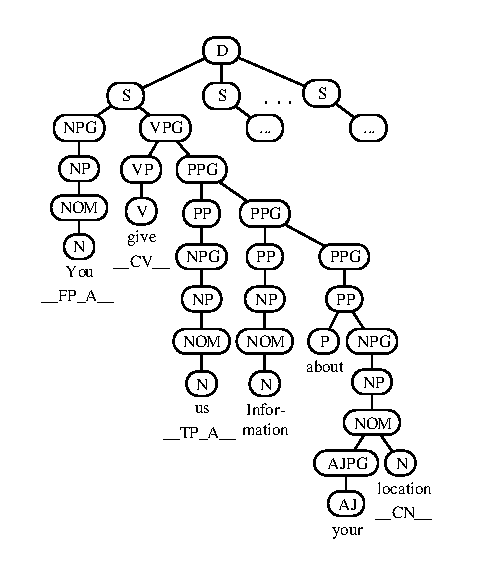
\includegraphics[width=.7\textwidth]{4.pdf}}
    \vspace{-\baselineskip}
\end{figure}

Здесь на рисунке \ref{fig:tree} <<\_\_FP\_A\_\_>> - метка актора-обладателя персональных данных, <<\_\_TP\_A\_\_>> - третья сторона, <<\_\_CV\_\_>> - глагол сбора, <<\_\_CN\_\_>> - существительное сбора. Когда было построено дерево предложений последовательность меток ключевых слов может быть распознана. В этом случае представленная на рисунке \ref{fig:tree}, последовательность <<\_\_FP\_A\_\_>>, <<\_\_CV\_\_>>, <<\_\_CN\_\_>> хорошо видна. Такие атомарные последовательности, раскрывают значения частей предложения и могут быть объединены в список, после этого весь смысл документов будет описан этим список. Сочетание маркировки ключевых слов и синтаксического анализа дает значения ключевых слов с отношениями между этими словами, определенными в виде древовидных структур. Дерево структура данных более гибкая, чем строка предложения, деревья и особенно поддеревья показывают важные отношения между словами. Запросы к таким структурам могут дать необходимую информацию для построения логических последовательностей действующих лиц, их действий, субъектов этих действий и, наконец, обстоятельств. Предлагаемый подход определенно имеет такие недостатки, как низкая производительность, вручную определенные пулы синонимов и т.д.


В результате апробации алгоритма латентно-семантического анализа было выяснено что для кластеризации экстремально схожих между собой текстов он  подходит не лучшим образом. В связи с этими обстоятельствами было решено обратить внимание на несколько иной подход анализа текста, основанный на контекстно-свободных грамматиках, тегировании по частям речи и синонимическом поиске.

\subsection{Выводы по строгим методам текстового анализа}

Эксперименты показали, что оба рассмотренных метода имеют как преимущества, так и определенные недостатки. Хотя предложенные подходы, оказались противоречивыми, окончательные результаты заслуживают внимания. Подход с латентно-семантическим поиском оказался не слишком эффективным. Однако, подход основанный на грамматическом анализе предложений и синонимическом поиске дал определенные результаты. Хоть он и не является производительным, с его помощью возможно производить выделение логических цепочек из предложений для получения более формального описания политик безопасности нежели их текстовые варианты.

\subsection{Подход основанный на глубоком обучении}
Исходя из проведенных исследований стало понятно, что более предпочтительным вариантом решения задачи будет подход с применением моделей с глубоким обучением. Реализация подобного проекта -- комплексная задача, ее можно разделить на несколько этапов. Сначала необходимо собрать датасет, потом его разметить для обучения модели, далее обучить модель и получить результаты. Однако сбор датасета тоже является непростой задачей. Для того чтобы осуществить сбор датасета необходим инструмент для поиска и скачивания вэб-страниц из сети интернет. Затем необходимо произвести очистку данных, удалить все теги со страниц, чтобы можно было передать текст аннотаторам. Все этапы сбора датасета полагаются на базу данных. Она лишена сложного объектно-реляционного моделирования, так как в ней по сути необходимо только хранить промежуточные результаты обработки текстовых файлов.

\newpage
\section{Проектирование инструментария}

\subsection{Техническое задание <<Инструментарий для сбора датасета>>}

\subsubsection{Основные положения технического задания}

\subsubsection{Скрейпер вэб-страниц}
Скачивание веб-страниц будет производиться инструментом написанном на языке Python, с помощью библиотек можно скачивать страницы анализировать данные с них, переходить по гиперссылкам и много другое. Такой инструмент позволит просматривать и сохранять содержимое страниц в автоматическом режиме без вмешательства пользователя. Таким образом в автоматическом режиме можно сохранить и проанализировать огромное количество текстовой информации.

\subsubsection{Очистка скачанных страниц политик}
Для очистки страниц от кода разметки планируется использовать библиотеку <<html sanitizer>>. Очистка кода необходима для того, чтобы аннотаторы могли максимально сфокусироваться на анализе текста, таким образом получая чистый текст они не будут отвлекаться на не имеющие значения в контексте задачи фрагменты.

\subsubsection{Инструмент разметки датасета}
Инструмент разметки датасета планировалось реализовать с помощью веб-технологий. Серверная часть будет полагаться на приложение, написанное на PHP, которое будет регулировать порядок выдачи текста на аннотирование. Процесс разметки высокодинамичен, поэтому невозможно избежать написания качественной клиентской части приложения на языке javascript. Это позволит сделать работу аннотаторов максимально производительной, в <<одну сессию>>, так как страница не будет перезагружаться, однако все изменения, которые будут вносится, сохранятся.

\subsubsection{Фреймворк глубокого обучения}
Для создания и тренировки модели анализа текста планируется использовать фреймворк машинного обучения <<Keras>>. Он позволяет быстро создавать классификаторы с самыми разными конфигурациями и любых типов.

После того как классификатор будет сконфигурирован останется лишь обучить его на датасете, полученном ранее.

Обученный классификатор будет в состоянии определять различные характеристики политики безопасности и аспекты обращения с данными, что позволит в автоматическом режиме формировать краткие отчеты о безопасности предоставляемого соглашения.

\subsection{Первичная декомпозиция и планирование}
Начальным этапом решения задачи является первичная декомпозиция, в ее результате выделяются подзадачи различной важности, которые должны быть решены для доведения цикла разработки до конца. В данном случае можно выделить следующие подзадачи:
\begin{enumerate}
    \item определение источника информации о различной IoT-продукции,
    \item отправка поискового запроса,
    \item получение результатов запроса (список IoT-продуктов),
    \item определение производителей IoT-продукции,
    \item поиск официальных сайтов производителей в сети интернет,
    \item поиск раздела <<политика безопасности>> на сайтах производителей,
    \item скачивание политик безопасности,
    \item очистка скачанных веб-документов от лишних элементов разметки.
\end{enumerate}

Получение списка производителей возможно на электронных торговых площадках, типовая разметка веб-страниц располагает для получения такой информации, так как существует лишь несколько вариантов наполнения страницы продукции.

Получение официальных веб-сайтов производителей задача на первый взгляд сложная, однако результаты ручной проверки показали, что лучшим вариантом является поисковый запрос с названием производителя <<как есть>>. В таком случае веб-сайт производителя оказывается на первой строчке результата поискового запроса, а если не оказывается, значит у этой компании его с очень большой вероятностью нет.

\subsection{Приложение вэб-скрейпер}

\subsubsection{Структура приложения вэб-скрейпера}
Исходя из результатов декомпозиции, эффективным подходом выглядит представление приложения в виде последовательно выполняющихся подпрограмм так, что входом модуля является результат работы предыдуще\-го модуля, то есть в виде конвейера. Схема организации приложения предста\-влена на рисунке \ref{fig:pipeline}.

\begin{figure}[H]
    \centering
    \ffigbox[\FBwidth]
    {\caption{Схема организации приложения\label{fig:pipeline}}}
    {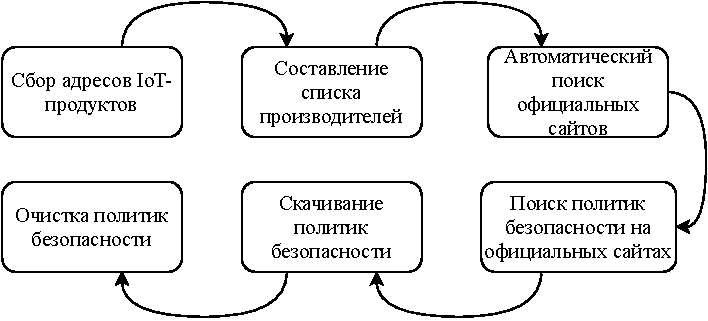
\includegraphics[width=\textwidth]{pics-pipeline.pdf}}
    \vspace{-\baselineskip}
\end{figure}

Далее была разработана композиционная модель приложения, на ней присутствуют все необходимые для решения задач модули. Схема представлена на рисунке \ref{fig:composition}.

\begin{figure}[H]
    \centering
    \ffigbox[\FBwidth]
    {\caption{Композиционная модель приложения\label{fig:composition}}}
    {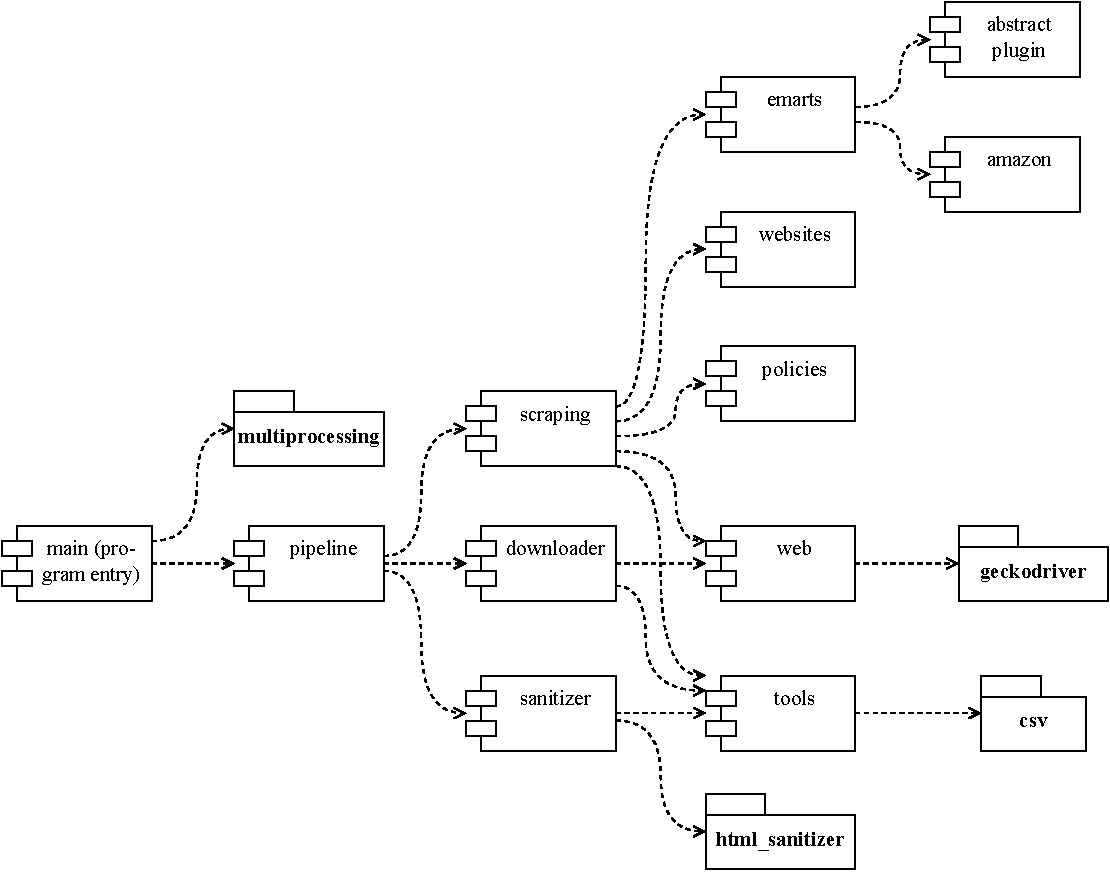
\includegraphics[width=\textwidth]{pics-modules.pdf}}
    \vspace{-\baselineskip}
\end{figure}

Здесь на рисунке \ref{fig:composition} модуль <<main>> отвечает за запуск программы, развертывание основных ее частей. Там же происходит инициализация пула потоков для мультипроцессинга затратных задач таких как, например, взаимодействие с <<безголовым>> браузером.

Модуль <<pipeline>> отвечает за последовательное исполнение подпрограмм элементов конвейера. Он осуществляет прием выходных и передачу входных данных.

Модуль <<scraping>> отвечает за получение данных с веб-страниц. Информация полученная с помощью этого модуля записывается в csv-файл для большей прозрачности и возможности сохранения результатов между запусками приложения, например, для пропуска данного этапа и использования его сохраненных результатов работы. Он включает в себя 3 основных действия:
\begin{enumerate}
    \item получение производителей IoT-продуктов (соответствует модулю <<e\-marts>>),
    \item получение официальных сайтов производителей (соответствует модулю <<websites>>),
    \item получение веб-ссылок на политики безопасности (соответствует модулю <<policies>>).
\end{enumerate}

Модуль <<downloader>> отвечает за скачивание страниц и их сохранение в отведенную для этого директорию. Информация полученная с помощью этого модуля записывается в html-файлы для большей прозрачности и возможности сохранения результатов между запусками приложения, например, для пропуска данного этапа и использования его сохраненных результатов работы.

Модуль <<sanitizer>> отвечает за очистку скачанных веб-страниц от не\-нужных тегов и ссылок. Информация полученная с помощью этого модуля записывается в html-файлы для большей прозрачности и возможности сохранения результатов между запусками приложения, например, для пропуска данного этапа и использования его сохраненных результатов работы.

Модуль <<emarts>> включает в себя набор плагинов, каждый из которых адаптирован для получения требуемой информации с определенного шаблона веб-страничной разметки. Некоторое поведение инкапсулировано в абстрактном плагине для увеличения <<reusability>> кода. Получая адрес на вход, данный плагин производит скачивание страницы и с помощью набора шаблонов пытается извлечь информацию. Данный модуль записывает полученную с помощью плагинов информацию в csv-файл для большей прозрачности и возможности сохранения результатов между запусками приложения, например, для пропуска данного этапа и использования его сохраненных результатов работы.

Модуль <<web>> отвечает за взаимодействие с веб-сайтами будь то торговые площадки или сайты производителей IoT-продуктов. В нем используется geckodriver для управления <<безголовым>> браузером.

Модуль <<tools>> содержит вспомогательные функции, в частности для ввода и вывода данных в формате csv.

\subsubsection{Потенциальные проблемы}
Потенциально возможные проблемы при реализации приложений подобного типа:
\begin{enumerate}
    \item блокировка из-за подозрительных заголовков браузера,
    \item блокировка из-за слишком частого обращения с запросами,
    \item как следствие 2-х предыдущих пунктов требование подтвердить, что это не попытка автоматического доступа (ввод капчи).
\end{enumerate}

Упомянутые проблемы решаются использованием разных заголовков браузера попеременно. Также отправка запросов ограничена по частоте от 15 до 30 секунд, ограничение выбирается случайным образом. Такие решения позволяют крайне редко попадать под подозрения, соответственно процент успеха при попытке получить данные с веб-страницы значительно повышается.

\subsection{Инструмент разметки датасета}
Инструмент разметки датасета планировалось реализовать с помощью веб-технологий. Серверная часть будет полагаться на приложение, написанное на PHP, которое будет регулировать порядок выдачи текста на аннотирование. Процесс разметки высокодинамичен, поэтому невозможно избежать написания качественной клиентской части приложения на языке javascript. Это позволит сделать работу аннотаторов максимально производительной, в <<одну сессию>>, так как страница не будет перезагружаться, однако все изменения, которые будут вносится, сохранятся.

\subsubsection{Объектное моделирование приложения}

Объектная модель инструмента представлена на рисунке \ref{fig:object}.

\begin{figure}[H]
    \centering
    \ffigbox[\FBwidth]
    {\caption{Объектная модель\label{fig:object}}}
    {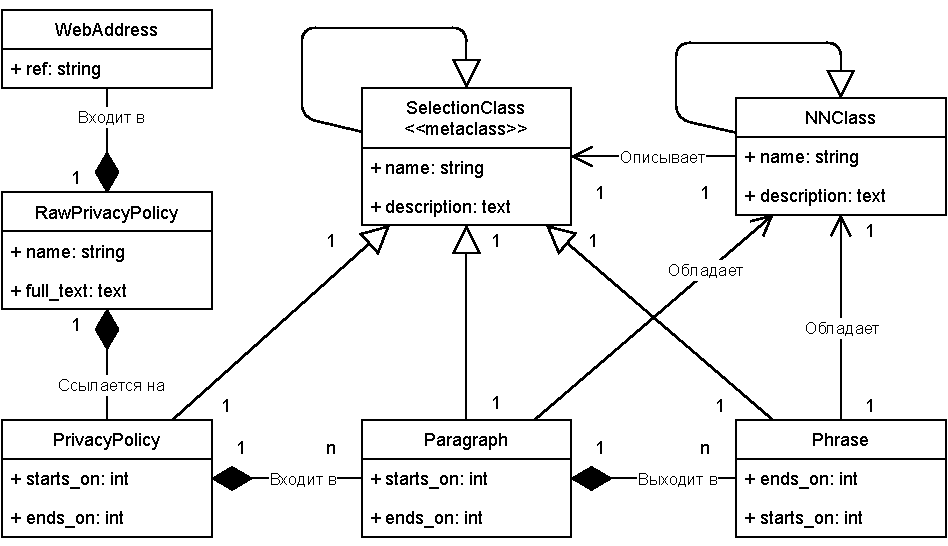
\includegraphics[width=.7\textwidth]{models-object.pdf}}
    \vspace{-\baselineskip}
\end{figure}

\subsubsection{Реляционная модель приложения}

Реляционная модель инструмента представлена на рисунке \ref{fig:relational}.

\begin{figure}[H]
    \centering
    \ffigbox[\FBwidth]
    {\caption{Реляционная модель\label{fig:relational}}}
    {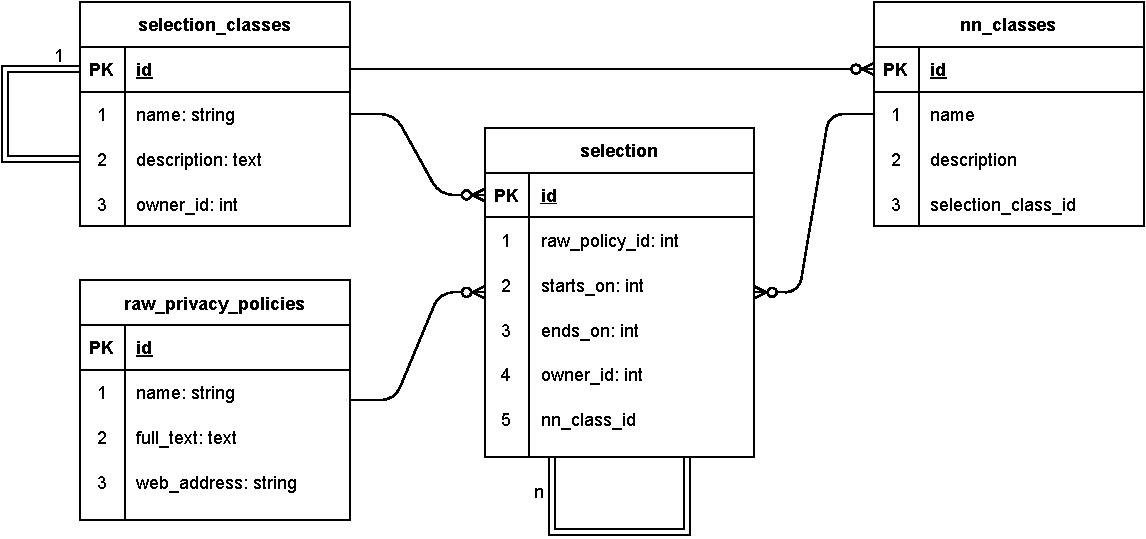
\includegraphics[width=.7\textwidth]{models-relational.pdf}}
    \vspace{-\baselineskip}
\end{figure}

\subsubsection{Проектирование пользовательского интерфейса}

Презентационный прототип интерфейса инструмента представлен на рисунке \ref{fig:proto}.

\begin{figure}[H]
    \centering
    \ffigbox[\FBwidth]
    {\caption{Презентационный прототип интерфейса\label{fig:proto}}}
    {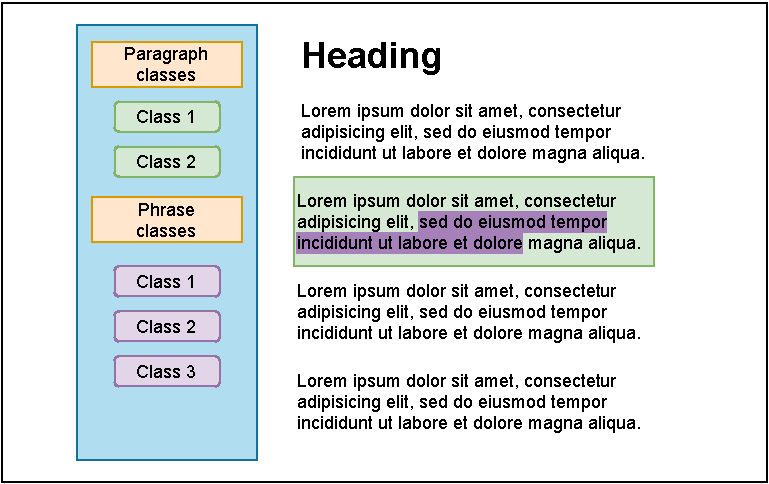
\includegraphics[width=.7\textwidth]{models-proto.pdf}}
    \vspace{-\baselineskip}
\end{figure}

\subsection{Выбор средств разработки}
Для реализации приложения были выбраны следующие средства:
\begin{enumerate}
    \item python 3.8.5,
    \item <<безголовый>> браузер Firefox,
    \item драйвер для управления <<безголовым>> браузером geckodriver,
    \item библиотека html sanitizer для очистки скачанных веб-документов.
\end{enumerate}
Выбор <<безголового>> браузера обусловлен потребностью в отрисовке страниц, так как на некоторых веб-страницах разметка генерируется с помощью javascript. Это делает невозможным использование простого скачивания, не\-обходима страница именно с исполненными скриптами, в противном случае будет невозможно получить требуемую информацию. В то же время браузер лишен графического интерфейса, чем снижается потребление вычислительных ресурсов.

\newpage
\section{Реализация инструментария}

\subsection{Полученные в результате реализации исходные коды}
В соответствии с результатами декомпозиции, выбора средств и проектирования приложение было реализовано. Характеристики полученных классов и функций приведены далее, в таблицах ?-?. Исходные коды представлены в приложении \hyperref[sec:appendix]{А}.

\subsection{Полученный в результате реализации пользовательский интерфейс инструмента разметки}

\subsection{Результаты решения поставленной задачи с помощью разработанного инструментария}
В результате работы программы были найдены 65 политик безопасности, разумеется среди них имеется определенный процент промахов, если производитель имеет сходство с каким либо другим более крупным. Поиск осуществлялся по торговой площадке amazon, брались результаты поискового запроса по первым 10-ти страницам, по категориям <<smart scales>>, <<smart watches>>, <<smart locks>> и <<smart bulbs>>. Всего производителей было найдено приблизительно 160. Стоит отметить, что результат является приемлемым, так как многие производители на данной торговой площадке не имеют выделенного веб-сайта, а пользуются услугами amazon, то есть на таких страницах действует политика безопасности amazon, а не производителя. Также стоит отметить что у некоторых продуктов явно не указан производитель, что сократило количественно результат поиска.

\end{document}